\documentclass[twoside]{book}

% Packages required by doxygen
\usepackage{fixltx2e}
\usepackage{calc}
\usepackage{doxygen}
\usepackage[export]{adjustbox} % also loads graphicx
\usepackage{graphicx}
\usepackage[utf8]{inputenc}
\usepackage{makeidx}
\usepackage{multicol}
\usepackage{multirow}
\PassOptionsToPackage{warn}{textcomp}
\usepackage{textcomp}
\usepackage[nointegrals]{wasysym}
\usepackage[table]{xcolor}

% Font selection
\usepackage[T1]{fontenc}
\usepackage[scaled=.90]{helvet}
\usepackage{courier}
\usepackage{amssymb}
\usepackage{sectsty}
\renewcommand{\familydefault}{\sfdefault}
\allsectionsfont{%
  \fontseries{bc}\selectfont%
  \color{darkgray}%
}
\renewcommand{\DoxyLabelFont}{%
  \fontseries{bc}\selectfont%
  \color{darkgray}%
}
\newcommand{\+}{\discretionary{\mbox{\scriptsize$\hookleftarrow$}}{}{}}

% Page & text layout
\usepackage{geometry}
\geometry{%
  a4paper,%
  top=2.5cm,%
  bottom=2.5cm,%
  left=2.5cm,%
  right=2.5cm%
}
\tolerance=750
\hfuzz=15pt
\hbadness=750
\setlength{\emergencystretch}{15pt}
\setlength{\parindent}{0cm}
\setlength{\parskip}{3ex plus 2ex minus 2ex}
\makeatletter
\renewcommand{\paragraph}{%
  \@startsection{paragraph}{4}{0ex}{-1.0ex}{1.0ex}{%
    \normalfont\normalsize\bfseries\SS@parafont%
  }%
}
\renewcommand{\subparagraph}{%
  \@startsection{subparagraph}{5}{0ex}{-1.0ex}{1.0ex}{%
    \normalfont\normalsize\bfseries\SS@subparafont%
  }%
}
\makeatother

% Headers & footers
\usepackage{fancyhdr}
\pagestyle{fancyplain}
\fancyhead[LE]{\fancyplain{}{\bfseries\thepage}}
\fancyhead[CE]{\fancyplain{}{}}
\fancyhead[RE]{\fancyplain{}{\bfseries\leftmark}}
\fancyhead[LO]{\fancyplain{}{\bfseries\rightmark}}
\fancyhead[CO]{\fancyplain{}{}}
\fancyhead[RO]{\fancyplain{}{\bfseries\thepage}}
\fancyfoot[LE]{\fancyplain{}{}}
\fancyfoot[CE]{\fancyplain{}{}}
\fancyfoot[RE]{\fancyplain{}{\bfseries\scriptsize Generated by Doxygen }}
\fancyfoot[LO]{\fancyplain{}{\bfseries\scriptsize Generated by Doxygen }}
\fancyfoot[CO]{\fancyplain{}{}}
\fancyfoot[RO]{\fancyplain{}{}}
\renewcommand{\footrulewidth}{0.4pt}
\renewcommand{\chaptermark}[1]{%
  \markboth{#1}{}%
}
\renewcommand{\sectionmark}[1]{%
  \markright{\thesection\ #1}%
}

% Indices & bibliography
\usepackage{natbib}
\usepackage[titles]{tocloft}
\setcounter{tocdepth}{3}
\setcounter{secnumdepth}{5}
\makeindex

% Hyperlinks (required, but should be loaded last)
\usepackage{ifpdf}
\ifpdf
  \usepackage[pdftex,pagebackref=true]{hyperref}
\else
  \usepackage[ps2pdf,pagebackref=true]{hyperref}
\fi
\hypersetup{%
  colorlinks=true,%
  linkcolor=blue,%
  citecolor=blue,%
  unicode%
}

% Custom commands
\newcommand{\clearemptydoublepage}{%
  \newpage{\pagestyle{empty}\cleardoublepage}%
}

\usepackage{caption}
\captionsetup{labelsep=space,justification=centering,font={bf},singlelinecheck=off,skip=4pt,position=top}

%===== C O N T E N T S =====

\begin{document}

% Titlepage & ToC
\hypersetup{pageanchor=false,
             bookmarksnumbered=true,
             pdfencoding=unicode
            }
\pagenumbering{alph}
\begin{titlepage}
\vspace*{7cm}
\begin{center}%
{\Large R\+P\+\_\+test \\[1ex]\large 0.\+1.\+0 }\\
\vspace*{1cm}
{\large Generated by Doxygen 1.8.14}\\
\end{center}
\end{titlepage}
\clearemptydoublepage
\pagenumbering{roman}
\tableofcontents
\clearemptydoublepage
\pagenumbering{arabic}
\hypersetup{pageanchor=true}

%--- Begin generated contents ---
\chapter{Hierarchical Index}
\section{Class Hierarchy}
This inheritance list is sorted roughly, but not completely, alphabetically\+:\begin{DoxyCompactList}
\item Test\begin{DoxyCompactList}
\item \contentsline{section}{Mrpt\+Test}{\pageref{class_mrpt_test}}{}
\item \contentsline{section}{Mrpt\+Test}{\pageref{class_mrpt_test}}{}
\item \contentsline{section}{Utility\+Test}{\pageref{class_utility_test}}{}
\end{DoxyCompactList}
\end{DoxyCompactList}

\chapter{Class Index}
\section{Class List}
Here are the classes, structs, unions and interfaces with brief descriptions\+:\begin{DoxyCompactList}
\item\contentsline{section}{\mbox{\hyperlink{class_mrpt_test}{Mrpt\+Test}} }{\pageref{class_mrpt_test}}{}
\item\contentsline{section}{\mbox{\hyperlink{class_utility_test}{Utility\+Test}} }{\pageref{class_utility_test}}{}
\end{DoxyCompactList}

\chapter{Class Documentation}
\hypertarget{class_mrpt_test}{}\section{Mrpt\+Test Class Reference}
\label{class_mrpt_test}\index{Mrpt\+Test@{Mrpt\+Test}}
Inheritance diagram for Mrpt\+Test\+:\begin{figure}[H]
\begin{center}
\leavevmode
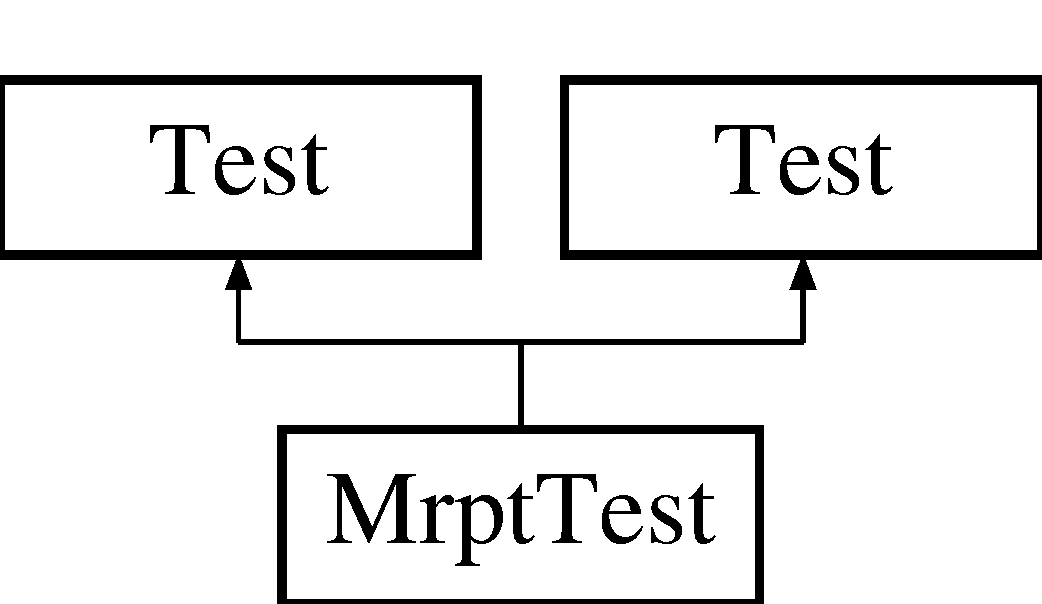
\includegraphics[height=2.000000cm]{class_mrpt_test}
\end{center}
\end{figure}
\subsection*{Protected Member Functions}
\begin{DoxyCompactItemize}
\item 
float \mbox{\hyperlink{class_mrpt_test_a37d1f6f738de308f759d1969e5027331}{get\+Split\+Point}} (const Mrpt \&mrpt, int tree, int index)
\item 
int \mbox{\hyperlink{class_mrpt_test_a0f86fdf9acb69beaf6ba83bdb612328f}{get\+Leaf\+Point}} (const Mrpt \&mrpt, int tree, int leaf, int index)
\item 
int \mbox{\hyperlink{class_mrpt_test_a2f93e8ec8143904d8a8a0989e46c8e07}{get\+Leaf\+Size}} (const Mrpt \&mrpt, int tree, int leaf) const
\item 
\mbox{\Hypertarget{class_mrpt_test_a7dadfb119a316b717a938b16eba5a85d}\label{class_mrpt_test_a7dadfb119a316b717a938b16eba5a85d}} 
void {\bfseries autotuning\+Grow\+Tester} (float density, int trees\+\_\+max, int depth\+\_\+max, int depth\+\_\+min, int votes\+\_\+max, int k)
\item 
\mbox{\Hypertarget{class_mrpt_test_a9c021901ef30d7752bb775ed2b6518c8}\label{class_mrpt_test_a9c021901ef30d7752bb775ed2b6518c8}} 
void {\bfseries autotuning\+Tester} (double target\+\_\+recall, float density, int trees\+\_\+max)
\item 
\mbox{\Hypertarget{class_mrpt_test_a03447daf507f3d177cc5496e08fcc3e1}\label{class_mrpt_test_a03447daf507f3d177cc5496e08fcc3e1}} 
void {\bfseries default\+Argument\+Tester} (int k)
\item 
\mbox{\Hypertarget{class_mrpt_test_af0d2e00bf524098a7a4af64c8b2cce79}\label{class_mrpt_test_af0d2e00bf524098a7a4af64c8b2cce79}} 
void {\bfseries test\+Parameters} (const Mrpt\+\_\+\+Parameters \&par, const Mrpt\+\_\+\+Parameters \&par2)
\item 
\mbox{\Hypertarget{class_mrpt_test_ad68f94de06a721657acaf486ccf59fed}\label{class_mrpt_test_ad68f94de06a721657acaf486ccf59fed}} 
void {\bfseries test\+Optimal\+Parameters} (const std\+::vector$<$ Mrpt\+\_\+\+Parameters $>$ \&pars, const std\+::vector$<$ Mrpt\+\_\+\+Parameters $>$ \&pars2)
\item 
\mbox{\Hypertarget{class_mrpt_test_a49fc9f53a471d9cb4d2757a2153e66a5}\label{class_mrpt_test_a49fc9f53a471d9cb4d2757a2153e66a5}} 
void {\bfseries save\+Tester} (int n\+\_\+trees, int depth, float density, int seed\+\_\+mrpt)
\item 
\mbox{\Hypertarget{class_mrpt_test_ae321902a9a99a5273e217142c433ad8b}\label{class_mrpt_test_ae321902a9a99a5273e217142c433ad8b}} 
void {\bfseries save\+Tester\+Autotuning} (int k, int trees\+\_\+max, int depth\+\_\+max, int depth\+\_\+min, int votes\+\_\+max, float density, int seed\+\_\+mrpt)
\item 
\mbox{\Hypertarget{class_mrpt_test_af4950dfd57a1ca45b864e0d93e2e5613}\label{class_mrpt_test_af4950dfd57a1ca45b864e0d93e2e5613}} 
void {\bfseries save\+Tester\+Autotuning\+Target\+Recall} (double target\+\_\+recall, int k, int trees\+\_\+max, int depth\+\_\+max, int depth\+\_\+min, int votes\+\_\+max, float density, int seed\+\_\+mrpt)
\item 
\mbox{\Hypertarget{class_mrpt_test_a4d0c6652a6b8b7e23fc462e2c1915ac6}\label{class_mrpt_test_a4d0c6652a6b8b7e23fc462e2c1915ac6}} 
void {\bfseries query\+Tester} (int n\+\_\+trees, int depth, float density, int votes, int k)
\item 
\mbox{\Hypertarget{class_mrpt_test_a1621d2f00e83347acf08c1ab149676dc}\label{class_mrpt_test_a1621d2f00e83347acf08c1ab149676dc}} 
void {\bfseries split\+Points\+Equal} (Mrpt \&mrpt1, Mrpt \&mrpt2)
\item 
\mbox{\Hypertarget{class_mrpt_test_a92177af2ff7703a6e918d8a2657c3a8c}\label{class_mrpt_test_a92177af2ff7703a6e918d8a2657c3a8c}} 
void {\bfseries leaves\+Equal} (Mrpt \&mrpt1, Mrpt \&mrpt2)
\item 
\mbox{\Hypertarget{class_mrpt_test_a3e5e1209e8780954de1dd64355097399}\label{class_mrpt_test_a3e5e1209e8780954de1dd64355097399}} 
Matrix\+Xi {\bfseries compute\+Exact\+Neighbors} (const Matrix\+Xf \&query, const Matrix\+Xf \&data)
\item 
\mbox{\Hypertarget{class_mrpt_test_aa3de00bf750bed73b893959bea7d680b}\label{class_mrpt_test_aa3de00bf750bed73b893959bea7d680b}} 
void {\bfseries print\+Parameters} (const Mrpt\+\_\+\+Parameters \&op)
\item 
\mbox{\Hypertarget{class_mrpt_test_af6e587c4f3c7d31719b40685fbedc61b}\label{class_mrpt_test_af6e587c4f3c7d31719b40685fbedc61b}} 
double {\bfseries get\+Recall} (std\+::vector$<$ std\+::vector$<$ int $>$$>$ results, Matrix\+Xi exact)
\item 
\mbox{\Hypertarget{class_mrpt_test_a64456333c8478e6c1d33d922b467d8f8}\label{class_mrpt_test_a64456333c8478e6c1d33d922b467d8f8}} 
std\+::vector$<$ std\+::vector$<$ int $>$ $>$ {\bfseries normal\+Query} (const Mrpt \&mrpt, int k, int v)
\item 
\mbox{\Hypertarget{class_mrpt_test_a9f4e07d231e79a00f9d84d4e0fbdf5db}\label{class_mrpt_test_a9f4e07d231e79a00f9d84d4e0fbdf5db}} 
std\+::vector$<$ std\+::vector$<$ int $>$ $>$ {\bfseries normal\+Query\+Vector} (const Mrpt \&mrpt, int k, int v)
\item 
\mbox{\Hypertarget{class_mrpt_test_aee2dbc061d3abacb21159eaab9265ed9}\label{class_mrpt_test_aee2dbc061d3abacb21159eaab9265ed9}} 
std\+::vector$<$ std\+::vector$<$ int $>$ $>$ {\bfseries normal\+Query\+Float\+Pointer} (const Mrpt \&mrpt, int k, int v)
\item 
\mbox{\Hypertarget{class_mrpt_test_accc9a4b0741f6a8fd4478fbfd6a7c216}\label{class_mrpt_test_accc9a4b0741f6a8fd4478fbfd6a7c216}} 
std\+::vector$<$ std\+::vector$<$ int $>$ $>$ {\bfseries autotuning\+Query} (const Mrpt \&mrpt)
\item 
\mbox{\Hypertarget{class_mrpt_test_af39bc82becae6e97df569dafd13ff7ef}\label{class_mrpt_test_af39bc82becae6e97df569dafd13ff7ef}} 
std\+::vector$<$ std\+::vector$<$ int $>$ $>$ {\bfseries autotuning\+Query\+Vector} (const Mrpt \&mrpt)
\item 
\mbox{\Hypertarget{class_mrpt_test_a0fcd1342fd53c2d6ad4320ce2999d463}\label{class_mrpt_test_a0fcd1342fd53c2d6ad4320ce2999d463}} 
std\+::vector$<$ std\+::vector$<$ int $>$ $>$ {\bfseries autotuning\+Query\+Float\+Pointer} (const Mrpt \&mrpt)
\item 
\mbox{\Hypertarget{class_mrpt_test_a52674dab297ed7341c36d4f490abd840}\label{class_mrpt_test_a52674dab297ed7341c36d4f490abd840}} 
std\+::vector$<$ std\+::vector$<$ int $>$ $>$ {\bfseries autotuning\+Query} (const Mrpt \&mrpt, double target\+\_\+recall)
\item 
\mbox{\Hypertarget{class_mrpt_test_a39620721d6847d06804c6e5d1fa8b323}\label{class_mrpt_test_a39620721d6847d06804c6e5d1fa8b323}} 
std\+::vector$<$ std\+::vector$<$ int $>$ $>$ {\bfseries autotuning\+Query\+Vector} (const Mrpt \&mrpt, double target\+\_\+recall)
\item 
\mbox{\Hypertarget{class_mrpt_test_ae7e6fd5653118328e9ba55dc134f8892}\label{class_mrpt_test_ae7e6fd5653118328e9ba55dc134f8892}} 
std\+::vector$<$ std\+::vector$<$ int $>$ $>$ {\bfseries autotuning\+Query\+Float\+Pointer} (const Mrpt \&mrpt, double target\+\_\+recall)
\item 
\mbox{\Hypertarget{class_mrpt_test_a45342980c86c0e7fdc857261aff805d6}\label{class_mrpt_test_a45342980c86c0e7fdc857261aff805d6}} 
void {\bfseries normal\+Query\+Equals} (const Mrpt \&mrpt1, const Mrpt \&mrpt2, int k, int v)
\item 
\mbox{\Hypertarget{class_mrpt_test_a5cd5276a3179c8263a918b00b3706a1d}\label{class_mrpt_test_a5cd5276a3179c8263a918b00b3706a1d}} 
void {\bfseries autotuning\+Query\+Equals} (const Mrpt \&mrpt1, const Mrpt \&mrpt2)
\item 
\mbox{\Hypertarget{class_mrpt_test_abb7c8b29bbe347a23afe4c52e38d7b69}\label{class_mrpt_test_abb7c8b29bbe347a23afe4c52e38d7b69}} 
void {\bfseries autotuning\+Query\+Equals} (const Mrpt \&mrpt1, const Mrpt \&mrpt2, double target\+\_\+recall)
\item 
\mbox{\Hypertarget{class_mrpt_test_a8992aa805af636a8bd77e358316ef5af}\label{class_mrpt_test_a8992aa805af636a8bd77e358316ef5af}} 
void {\bfseries exact\+Knn\+Equals} (const std\+::vector$<$ int $>$ \&result, const std\+::vector$<$ float $>$ \&distances)
\item 
\mbox{\Hypertarget{class_mrpt_test_a8d963c2338fa9897a1d7c26ec4b3b5c9}\label{class_mrpt_test_a8d963c2338fa9897a1d7c26ec4b3b5c9}} 
void {\bfseries private\+Exact\+Knn\+Tester} (int k)
\item 
\mbox{\Hypertarget{class_mrpt_test_ab6e235b8f4ab22e556f56ca5353c9aa3}\label{class_mrpt_test_ab6e235b8f4ab22e556f56ca5353c9aa3}} 
void {\bfseries exact\+Knn\+Tester} (int k)
\item 
\mbox{\Hypertarget{class_mrpt_test_a678906f353d1be1737679b8033ceb7c5}\label{class_mrpt_test_a678906f353d1be1737679b8033ceb7c5}} 
void {\bfseries vector\+Exact\+Knn\+Tester} (int k)
\item 
\mbox{\Hypertarget{class_mrpt_test_ac35674e85cc46d9760b8a9a28231ce25}\label{class_mrpt_test_ac35674e85cc46d9760b8a9a28231ce25}} 
void {\bfseries float\+Pointer\+Exact\+Knn\+Tester} (int k)
\item 
\mbox{\Hypertarget{class_mrpt_test_a0eec2104b55243ab2206ff4f40427c2f}\label{class_mrpt_test_a0eec2104b55243ab2206ff4f40427c2f}} 
void {\bfseries static\+Exact\+Knn\+Tester} (int k)
\item 
\mbox{\Hypertarget{class_mrpt_test_adfec34015157e7f3fa74aed98112fd4b}\label{class_mrpt_test_adfec34015157e7f3fa74aed98112fd4b}} 
void {\bfseries static\+Vector\+Exact\+Knn\+Tester} (int k)
\item 
\mbox{\Hypertarget{class_mrpt_test_aa18fe7f1c1e9519d110a09fa5ec91cbc}\label{class_mrpt_test_aa18fe7f1c1e9519d110a09fa5ec91cbc}} 
void {\bfseries static\+Float\+Pointer\+Exact\+Knn\+Tester} (int k)
\item 
\mbox{\Hypertarget{class_mrpt_test_ad3684771dbd14e1a612c772a47384137}\label{class_mrpt_test_ad3684771dbd14e1a612c772a47384137}} 
std\+::vector$<$ int $>$ {\bfseries get\+True\+Knn} (const Vector\+Xf \&query, const Matrix\+Xf \&data, std\+::vector$<$ float $>$ \&true\+\_\+distances)
\item 
\mbox{\Hypertarget{class_mrpt_test_acd205c7d3a12483c14ea4cc339245ece}\label{class_mrpt_test_acd205c7d3a12483c14ea4cc339245ece}} 
void {\bfseries generate\+\_\+x} (std\+::vector$<$ int $>$ \&x, int max\+\_\+generated, int n\+\_\+tested, int max\+\_\+val)
\item 
\mbox{\Hypertarget{class_mrpt_test_aadaa186b000780b4fca26e5b1c047702}\label{class_mrpt_test_aadaa186b000780b4fca26e5b1c047702}} 
void {\bfseries prune} (Mrpt \&mrpt, double target\+\_\+recall)
\item 
float \mbox{\hyperlink{class_mrpt_test_a37d1f6f738de308f759d1969e5027331}{get\+Split\+Point}} (const Mrpt \&mrpt, int tree, int index)
\item 
int \mbox{\hyperlink{class_mrpt_test_a0f86fdf9acb69beaf6ba83bdb612328f}{get\+Leaf\+Point}} (const Mrpt \&mrpt, int tree, int leaf, int index)
\item 
int \mbox{\hyperlink{class_mrpt_test_a2f93e8ec8143904d8a8a0989e46c8e07}{get\+Leaf\+Size}} (const Mrpt \&mrpt, int tree, int leaf) const
\item 
\mbox{\Hypertarget{class_mrpt_test_ac43a291223d3b284a0a527f805dfccc8}\label{class_mrpt_test_ac43a291223d3b284a0a527f805dfccc8}} 
void {\bfseries query\+Tester} (int n\+\_\+trees, int depth, float density, int votes, int k, std\+::vector$<$ int $>$ approximate\+\_\+knn)
\item 
\mbox{\Hypertarget{class_mrpt_test_a5df8b454cd02d3f640b3110b6abf4195}\label{class_mrpt_test_a5df8b454cd02d3f640b3110b6abf4195}} 
void {\bfseries test\+Split\+Points} (Mrpt \&index, Mrpt\+\_\+old \&index\+\_\+old)
\item 
\mbox{\Hypertarget{class_mrpt_test_a4953cebe12af6793be652c2342173a37}\label{class_mrpt_test_a4953cebe12af6793be652c2342173a37}} 
void {\bfseries split\+Point\+Tester} (int n\+\_\+trees, int depth, float density)
\item 
\mbox{\Hypertarget{class_mrpt_test_ad311f610823f0cd3f0100a78e74d4707}\label{class_mrpt_test_ad311f610823f0cd3f0100a78e74d4707}} 
void {\bfseries test\+Leaves} (Mrpt \&index, Mrpt\+\_\+old \&index\+\_\+old)
\item 
\mbox{\Hypertarget{class_mrpt_test_aff26535eb9b85211d23f291ed8e26d3f}\label{class_mrpt_test_aff26535eb9b85211d23f291ed8e26d3f}} 
void {\bfseries leaf\+Tester} (int n\+\_\+trees, int depth, float density)
\end{DoxyCompactItemize}
\subsection*{Protected Attributes}
\begin{DoxyCompactItemize}
\item 
\mbox{\Hypertarget{class_mrpt_test_a8d0a86d51be20dc97328d01ae3063f4d}\label{class_mrpt_test_a8d0a86d51be20dc97328d01ae3063f4d}} 
int {\bfseries d}
\item 
\mbox{\Hypertarget{class_mrpt_test_ab1668136de88087a8ae2a5c1082dec5d}\label{class_mrpt_test_ab1668136de88087a8ae2a5c1082dec5d}} 
int {\bfseries n}
\item 
\mbox{\Hypertarget{class_mrpt_test_a1c2e9b308d5e90fe1725e392efbeca13}\label{class_mrpt_test_a1c2e9b308d5e90fe1725e392efbeca13}} 
int {\bfseries n2}
\item 
\mbox{\Hypertarget{class_mrpt_test_a6a22d44b33026bca9a3ff546bdd17dfb}\label{class_mrpt_test_a6a22d44b33026bca9a3ff546bdd17dfb}} 
int {\bfseries n\+\_\+test}
\item 
\mbox{\Hypertarget{class_mrpt_test_ab1c4fae453c57ae3c53f46502750fabe}\label{class_mrpt_test_ab1c4fae453c57ae3c53f46502750fabe}} 
int {\bfseries seed\+\_\+data}
\item 
\mbox{\Hypertarget{class_mrpt_test_adc2cf40774fb479b1d1cbc9b453b329b}\label{class_mrpt_test_adc2cf40774fb479b1d1cbc9b453b329b}} 
int {\bfseries seed\+\_\+mrpt}
\item 
\mbox{\Hypertarget{class_mrpt_test_a645e29f102abc83e083fc8784547c434}\label{class_mrpt_test_a645e29f102abc83e083fc8784547c434}} 
double {\bfseries epsilon} = 0.\+001
\item 
\mbox{\Hypertarget{class_mrpt_test_a4db9dc6194b03b07f828eddbee4802e9}\label{class_mrpt_test_a4db9dc6194b03b07f828eddbee4802e9}} 
Matrix\+Xf {\bfseries X}
\item 
\mbox{\Hypertarget{class_mrpt_test_a4dc5308db9f91b5ccef42c4ec29a6a44}\label{class_mrpt_test_a4dc5308db9f91b5ccef42c4ec29a6a44}} 
Matrix\+Xf {\bfseries X2}
\item 
\mbox{\Hypertarget{class_mrpt_test_a486327c97fd0190be0d4ccb17be995de}\label{class_mrpt_test_a486327c97fd0190be0d4ccb17be995de}} 
Matrix\+Xf {\bfseries Q}
\item 
\mbox{\Hypertarget{class_mrpt_test_a63ad020a987a1de41bb1e6b435ec093e}\label{class_mrpt_test_a63ad020a987a1de41bb1e6b435ec093e}} 
Vector\+Xf {\bfseries q}
\item 
\mbox{\Hypertarget{class_mrpt_test_a21c057ee87babe0d71188e2c8abe549d}\label{class_mrpt_test_a21c057ee87babe0d71188e2c8abe549d}} 
Map$<$ const Matrix\+Xf $>$ {\bfseries M}
\item 
\mbox{\Hypertarget{class_mrpt_test_aa144675bd97f66a9bbc99f9000817b9e}\label{class_mrpt_test_aa144675bd97f66a9bbc99f9000817b9e}} 
Map$<$ const Matrix\+Xf $>$ {\bfseries M2}
\item 
\mbox{\Hypertarget{class_mrpt_test_a926776501a519880425e8f96573e719e}\label{class_mrpt_test_a926776501a519880425e8f96573e719e}} 
Map$<$ const Matrix\+Xf $>$ {\bfseries test\+\_\+queries}
\item 
\mbox{\Hypertarget{class_mrpt_test_aecfd31ef605ec06fa0c25d5dc6a3cd22}\label{class_mrpt_test_aecfd31ef605ec06fa0c25d5dc6a3cd22}} 
std\+::vector$<$ float $>$ {\bfseries true\+\_\+distances}
\item 
\mbox{\Hypertarget{class_mrpt_test_a92b151c5588efad4332e73ca921e68be}\label{class_mrpt_test_a92b151c5588efad4332e73ca921e68be}} 
std\+::vector$<$ int $>$ {\bfseries true\+\_\+knn}
\item 
\mbox{\Hypertarget{class_mrpt_test_a4a1d42172a04d98952c0002eb39eaf8d}\label{class_mrpt_test_a4a1d42172a04d98952c0002eb39eaf8d}} 
const Map$<$ const Matrix\+Xf $>$ $\ast$ {\bfseries M2\+\_\+pointer}
\end{DoxyCompactItemize}


\subsection{Member Function Documentation}
\mbox{\Hypertarget{class_mrpt_test_a0f86fdf9acb69beaf6ba83bdb612328f}\label{class_mrpt_test_a0f86fdf9acb69beaf6ba83bdb612328f}} 
\index{Mrpt\+Test@{Mrpt\+Test}!get\+Leaf\+Point@{get\+Leaf\+Point}}
\index{get\+Leaf\+Point@{get\+Leaf\+Point}!Mrpt\+Test@{Mrpt\+Test}}
\subsubsection{\texorpdfstring{get\+Leaf\+Point()}{getLeafPoint()}\hspace{0.1cm}{\footnotesize\ttfamily [1/2]}}
{\footnotesize\ttfamily int Mrpt\+Test\+::get\+Leaf\+Point (\begin{DoxyParamCaption}\item[{const Mrpt \&}]{mrpt,  }\item[{int}]{tree,  }\item[{int}]{leaf,  }\item[{int}]{index }\end{DoxyParamCaption})\hspace{0.3cm}{\ttfamily [inline]}, {\ttfamily [protected]}}

Accessor for point stored in leaves of trees (for testing purposes) 
\begin{DoxyParams}{Parameters}
{\em tree} & -\/ index of tree in (0, ... T-\/1) \\
\hline
{\em leaf} & -\/ index of leaf in (0, ... , 2$^\wedge$depth) \\
\hline
{\em index} & -\/ index of a data point in a leaf \\
\hline
\end{DoxyParams}
\begin{DoxyReturn}{Returns}
index of index\+:th data point in leaf\+:th leaf of tree\+:th tree 
\end{DoxyReturn}
\mbox{\Hypertarget{class_mrpt_test_a0f86fdf9acb69beaf6ba83bdb612328f}\label{class_mrpt_test_a0f86fdf9acb69beaf6ba83bdb612328f}} 
\index{Mrpt\+Test@{Mrpt\+Test}!get\+Leaf\+Point@{get\+Leaf\+Point}}
\index{get\+Leaf\+Point@{get\+Leaf\+Point}!Mrpt\+Test@{Mrpt\+Test}}
\subsubsection{\texorpdfstring{get\+Leaf\+Point()}{getLeafPoint()}\hspace{0.1cm}{\footnotesize\ttfamily [2/2]}}
{\footnotesize\ttfamily int Mrpt\+Test\+::get\+Leaf\+Point (\begin{DoxyParamCaption}\item[{const Mrpt \&}]{mrpt,  }\item[{int}]{tree,  }\item[{int}]{leaf,  }\item[{int}]{index }\end{DoxyParamCaption})\hspace{0.3cm}{\ttfamily [inline]}, {\ttfamily [protected]}}

Accessor for point stored in leaves of trees (for testing purposes) 
\begin{DoxyParams}{Parameters}
{\em tree} & -\/ index of tree in (0, ... T-\/1) \\
\hline
{\em leaf} & -\/ index of leaf in (0, ... , 2$^\wedge$depth) \\
\hline
{\em index} & -\/ index of a data point in a leaf \\
\hline
\end{DoxyParams}
\begin{DoxyReturn}{Returns}
index of index\+:th data point in leaf\+:th leaf of tree\+:th tree 
\end{DoxyReturn}
\mbox{\Hypertarget{class_mrpt_test_a2f93e8ec8143904d8a8a0989e46c8e07}\label{class_mrpt_test_a2f93e8ec8143904d8a8a0989e46c8e07}} 
\index{Mrpt\+Test@{Mrpt\+Test}!get\+Leaf\+Size@{get\+Leaf\+Size}}
\index{get\+Leaf\+Size@{get\+Leaf\+Size}!Mrpt\+Test@{Mrpt\+Test}}
\subsubsection{\texorpdfstring{get\+Leaf\+Size()}{getLeafSize()}\hspace{0.1cm}{\footnotesize\ttfamily [1/2]}}
{\footnotesize\ttfamily int Mrpt\+Test\+::get\+Leaf\+Size (\begin{DoxyParamCaption}\item[{const Mrpt \&}]{mrpt,  }\item[{int}]{tree,  }\item[{int}]{leaf }\end{DoxyParamCaption}) const\hspace{0.3cm}{\ttfamily [inline]}, {\ttfamily [protected]}}

Accessor for the number of points in a leaf of a tree (for test purposes) 
\begin{DoxyParams}{Parameters}
{\em tree} & -\/ index of tree in (0, ... T-\/1) \\
\hline
{\em leaf} & -\/ index of leaf in (0, ... , 2$^\wedge$depth) \\
\hline
\end{DoxyParams}
\begin{DoxyReturn}{Returns}
-\/ number of data points in leaf\+:th leaf of tree\+:th tree 
\end{DoxyReturn}
\mbox{\Hypertarget{class_mrpt_test_a2f93e8ec8143904d8a8a0989e46c8e07}\label{class_mrpt_test_a2f93e8ec8143904d8a8a0989e46c8e07}} 
\index{Mrpt\+Test@{Mrpt\+Test}!get\+Leaf\+Size@{get\+Leaf\+Size}}
\index{get\+Leaf\+Size@{get\+Leaf\+Size}!Mrpt\+Test@{Mrpt\+Test}}
\subsubsection{\texorpdfstring{get\+Leaf\+Size()}{getLeafSize()}\hspace{0.1cm}{\footnotesize\ttfamily [2/2]}}
{\footnotesize\ttfamily int Mrpt\+Test\+::get\+Leaf\+Size (\begin{DoxyParamCaption}\item[{const Mrpt \&}]{mrpt,  }\item[{int}]{tree,  }\item[{int}]{leaf }\end{DoxyParamCaption}) const\hspace{0.3cm}{\ttfamily [inline]}, {\ttfamily [protected]}}

Accessor for the number of points in a leaf of a tree (for test purposes) 
\begin{DoxyParams}{Parameters}
{\em tree} & -\/ index of tree in (0, ... T-\/1) \\
\hline
{\em leaf} & -\/ index of leaf in (0, ... , 2$^\wedge$depth) \\
\hline
\end{DoxyParams}
\begin{DoxyReturn}{Returns}
-\/ number of data points in leaf\+:th leaf of tree\+:th tree 
\end{DoxyReturn}
\mbox{\Hypertarget{class_mrpt_test_a37d1f6f738de308f759d1969e5027331}\label{class_mrpt_test_a37d1f6f738de308f759d1969e5027331}} 
\index{Mrpt\+Test@{Mrpt\+Test}!get\+Split\+Point@{get\+Split\+Point}}
\index{get\+Split\+Point@{get\+Split\+Point}!Mrpt\+Test@{Mrpt\+Test}}
\subsubsection{\texorpdfstring{get\+Split\+Point()}{getSplitPoint()}\hspace{0.1cm}{\footnotesize\ttfamily [1/2]}}
{\footnotesize\ttfamily float Mrpt\+Test\+::get\+Split\+Point (\begin{DoxyParamCaption}\item[{const Mrpt \&}]{mrpt,  }\item[{int}]{tree,  }\item[{int}]{index }\end{DoxyParamCaption})\hspace{0.3cm}{\ttfamily [inline]}, {\ttfamily [protected]}}

Accessor for split points of trees (for testing purposes) 
\begin{DoxyParams}{Parameters}
{\em tree} & -\/ index of tree in (0, ... , T-\/1) \\
\hline
{\em index} & -\/ the index of branch in (0, ... , (2$^\wedge$depth) -\/ 1)\+: 0 = root 1 = first branch of first level 2 = second branch of first level 3 = first branch of second level etc. \\
\hline
\end{DoxyParams}
\begin{DoxyReturn}{Returns}
split point of index\+:th branch of tree\+:th tree 
\end{DoxyReturn}
\mbox{\Hypertarget{class_mrpt_test_a37d1f6f738de308f759d1969e5027331}\label{class_mrpt_test_a37d1f6f738de308f759d1969e5027331}} 
\index{Mrpt\+Test@{Mrpt\+Test}!get\+Split\+Point@{get\+Split\+Point}}
\index{get\+Split\+Point@{get\+Split\+Point}!Mrpt\+Test@{Mrpt\+Test}}
\subsubsection{\texorpdfstring{get\+Split\+Point()}{getSplitPoint()}\hspace{0.1cm}{\footnotesize\ttfamily [2/2]}}
{\footnotesize\ttfamily float Mrpt\+Test\+::get\+Split\+Point (\begin{DoxyParamCaption}\item[{const Mrpt \&}]{mrpt,  }\item[{int}]{tree,  }\item[{int}]{index }\end{DoxyParamCaption})\hspace{0.3cm}{\ttfamily [inline]}, {\ttfamily [protected]}}

Accessor for split points of trees (for testing purposes) 
\begin{DoxyParams}{Parameters}
{\em tree} & -\/ index of tree in (0, ... , T-\/1) \\
\hline
{\em index} & -\/ the index of branch in (0, ... , (2$^\wedge$depth) -\/ 1)\+: 0 = root 1 = first branch of first level 2 = second branch of first level 3 = first branch of second level etc. \\
\hline
\end{DoxyParams}
\begin{DoxyReturn}{Returns}
split point of index\+:th branch of tree\+:th tree 
\end{DoxyReturn}


The documentation for this class was generated from the following files\+:\begin{DoxyCompactItemize}
\item 
test/test.\+cpp\item 
test/test\+\_\+implementation.\+cpp\end{DoxyCompactItemize}

\hypertarget{class_utility_test}{}\section{Utility\+Test Class Reference}
\label{class_utility_test}\index{Utility\+Test@{Utility\+Test}}
Inheritance diagram for Utility\+Test\+:\begin{figure}[H]
\begin{center}
\leavevmode
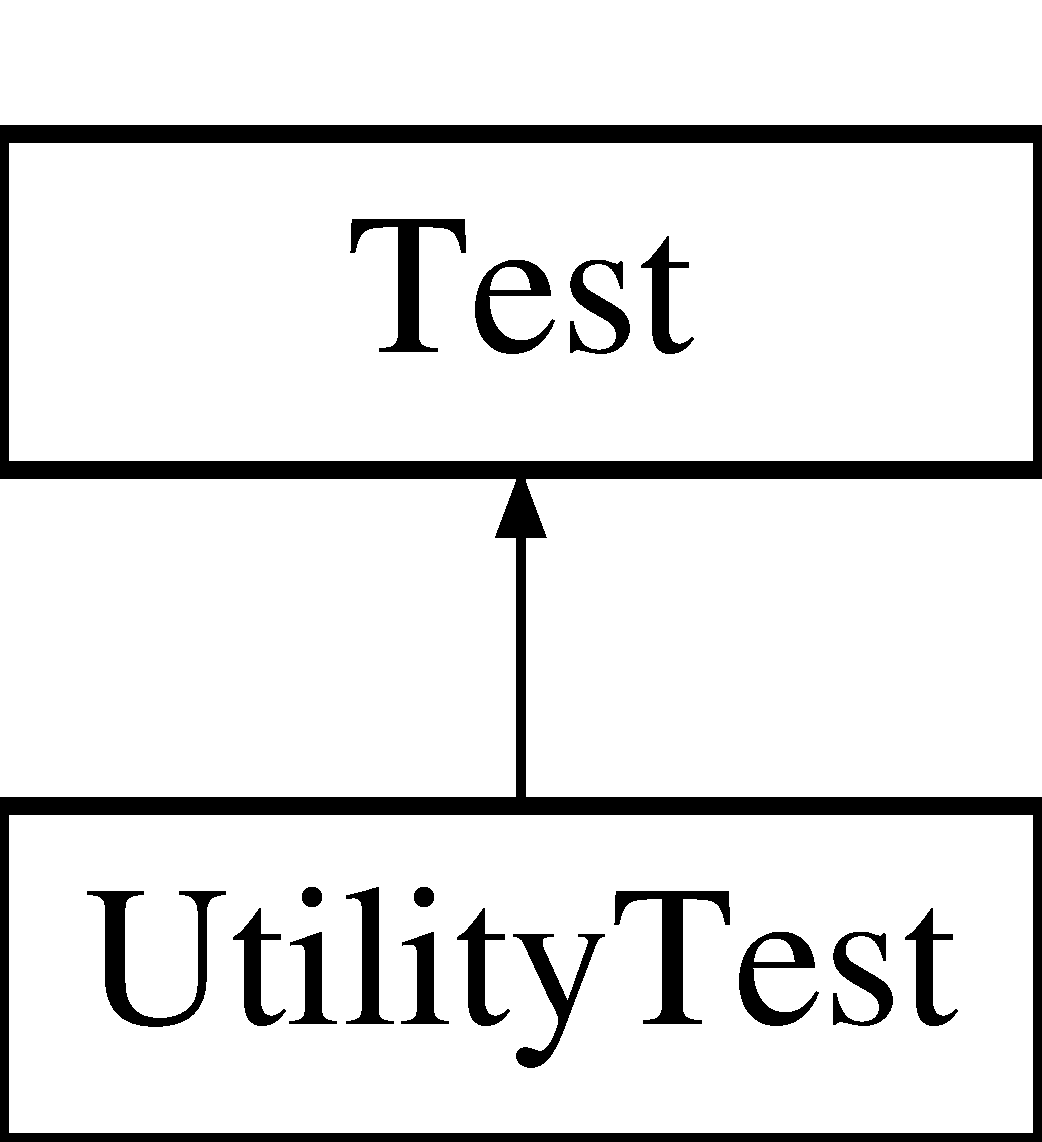
\includegraphics[height=2.000000cm]{class_utility_test}
\end{center}
\end{figure}
\subsection*{Protected Member Functions}
\begin{DoxyCompactItemize}
\item 
\mbox{\Hypertarget{class_utility_test_a2eb9bcd1dbd5eb5e2a35477ff7d80571}\label{class_utility_test_a2eb9bcd1dbd5eb5e2a35477ff7d80571}} 
void {\bfseries leaf\+Tester} (int n, int depth, const std\+::vector$<$ int $>$ \&indices\+\_\+reference)
\item 
\mbox{\Hypertarget{class_utility_test_ac195e9a5bada5bef6ea273ca6f7105d9}\label{class_utility_test_ac195e9a5bada5bef6ea273ca6f7105d9}} 
void {\bfseries all\+Leaves\+Tester} (int n, const std\+::vector$<$ std\+::vector$<$ int $>$$>$ \&indices\+\_\+reference)
\item 
\mbox{\Hypertarget{class_utility_test_af6666fec149c33f92bb64baa37d491c1}\label{class_utility_test_af6666fec149c33f92bb64baa37d491c1}} 
void {\bfseries test\+Theil\+Sen} (std\+::vector$<$ double $>$ x, std\+::vector$<$ double $>$ y, double intercept, double slope)
\end{DoxyCompactItemize}


The documentation for this class was generated from the following file\+:\begin{DoxyCompactItemize}
\item 
test/test.\+cpp\end{DoxyCompactItemize}

%--- End generated contents ---

% Index
\backmatter
\newpage
\phantomsection
\clearemptydoublepage
\addcontentsline{toc}{chapter}{Index}
\printindex

\end{document}
